\documentclass[tikz,border=5pt]{standalone}
\usepackage{tikz}
\usepackage{amsmath}
\begin{document}

\begin{figure}[H]
\centering
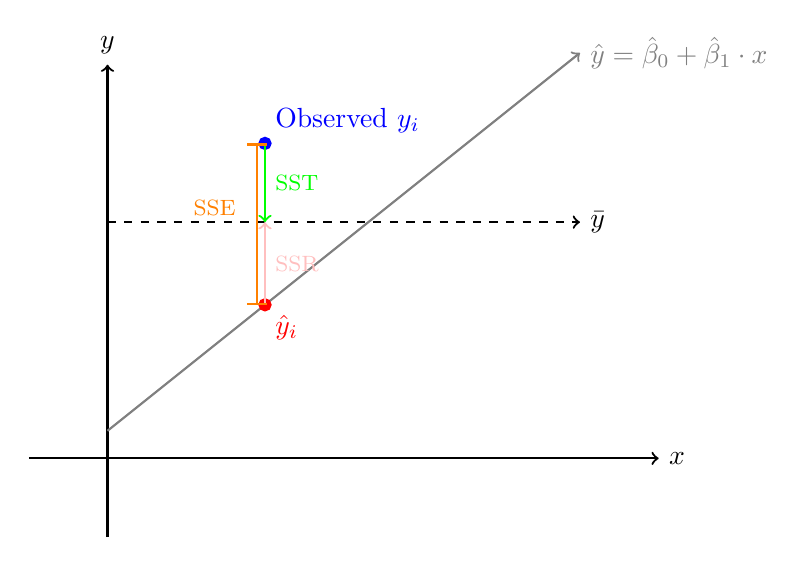
\begin{tikzpicture}[->, thick]
  \draw[->] (-1,0) -- (7,0) node[right] {$x$};
  \draw[->] (0,-1) -- (0,5) node[above] {$y$};
  \filldraw[blue] (2, 4) circle (2pt) node[above right] {Observed $y_i$};
  \draw[gray, thick, domain=0:6] plot (\x, {0.8*\x + 0.35}) node[right] {$\hat{y} = \hat{\beta}_0 + \hat{\beta}_1 \cdot x$};
  \draw[dashed] (0,3) -- (6,3) node[right] {$\bar{y}$};
  \coordinate (xhat) at (2, 1.95);
  \filldraw[red] (xhat) circle (2pt) node[below right] {$\hat{y}_i$};
  \draw[pink, thick] (xhat) -- (2, 3) node[midway, right] {\footnotesize SSR};
  \draw[green, thick] (2, 4) -- (2, 3) node[midway, right] {\footnotesize SST};
  \draw[thick, orange, |-|] (1.9, 1.95) -- (1.9, 4) node[midway, left=4pt, yshift=6pt] {\footnotesize SSE};

\end{tikzpicture}
\caption{Visual representation of regression variability. \textbf{SST} (green) is total variability from the mean, \textbf{SSR} (pink) is explained variability, and \textbf{SSE} (orange curly brace) is the residual (unexplained) variability between the observed value $y_i$ and the prediction $\hat{y}_i$.}
\end{figure}

\end{document}
